\documentclass[Softwaredesign/Softwaredesign_main.tex]{subfiles}
\begin{document}
\section{CupLight\_IF Hardware Design}
 I dette afsnit laves der overvejelser omkring det lys, der skal være under kopperne på Beer Pong bordet. Både lyset i al sin enkelthed men også hvordan lyset skal styres.
 
 
Før der dog kan laves et design, må der først og fremmest kigges på, hvilke krav der er til lyset. Af Kravsspecifikationen hives der følgende krav ud omkring lyset:
\begin{enumerate}
    \item Koplys skal kunne have forskellige farver.
    \item Hver enkelt koplys skal kunne styres individuelt, til at have sin egen farve.
\end{enumerate}
Da lyset skal styres af en controller pr. spillerside, så giver det umiddelbart også et krav om at alle led'er skal kunne styres med forholdsvis få pins på PSoC'en. 
\\Lyset skal kunne styres på en effektiv, men også billig måde, da det ville være spild af ressourcer at bruge al budgettet på bordet på at lave belysning frem for egentlig funktionalitet. Derfor besluttes der at bruge almindelige RGB-led'er, som kan købes på nettet forholdsvis billigt. 
\\Der findes to typer RGB-led'er; Common Anode og Common Cathode. Da der ikke er klare fordele og ulemper mellem de to, vælges en RGB-led med Common Cathode, da den har nogle fordele i forhold til den styring, der laves dertil.
\\Apropos styring, så kommer budgettet igen i spil, da styring, i så vidt muligt udfald, laves ud af komponenter, der er frit tilgængeligt\footnote{Obs. Komponenter der kan hentes i Lab på Ingeniør Højskolen}. 

\subsection{Design af LED Styring}
\subsubsection{Styring af RGB-led'er}
Det krav, der kommer til at vise sig ekstremt vigtigt og problematisk er kravet om, at hvert koplys skal kunne styres individuelt. En RGB-led har nemlig 4 ben, 1 ben til den røde farve, 1 ben til den grønne farve, 1 ben til den blå farve og 1 ben til katode/anode. Måden farven så styres på er, at man ved PWM ændrer spændingen på benene, og jo højere spænding jo kraftigere farve. Det er derfor intet problem at styre farverne på en LED, da der bare skal bruges 4 pins på PSoC'en, hvor en pin ved en transistor styrer om LED'en skal være tændt eller slukket og resten laver PWM. Men her bliver problemet også åbenlyst i det, der på hver playerside skal styres 6 forskellige lys. Hvis der altså ikke laves en anden løsning, så skal der bruges 24 pins bare til lys. 
\\Problemet kan umiddelbart løses ved multiplexing, dog gør denne løsning hardwaren lidt svære, og softwaren en del svære. Essensen i multiplexløsningen er, at LED'erne tændes hver især så hurtigt at det for menneskelige øjne ligner at LED'en lyser konstant. På den måde kan der bruges en fælles pin til henholdsvis rød, grøn og blå til alle led'er, samt en konstant mængde pins til at stå for multiplexing. Det vil altså sige, at alle led'er kan styres af en konstant mængde pins, hvilket også åbner op for, at der kan tilføjes et vilkårligt antal led'er, uden påvirkning af brugen af PSoC pins.
\\En anden måde til at kontrollere LED'erne, der blev taget i betragtning var det der kaldes Charlieplexing. Charlieplexing udnytter de 3 states på en microcontroller pin (High,Low,Input), til at kontrollere de givne LEDs. Denne metode ville helt klart være nemmest at implementere, da størstedelen er software, men desværre er det kun muligt at opnå 7 farver: Rød, Grøn, blå, gul, magenta, cyan og hvid. Der ønskes altså en løsning, hvor et højere spektrum af farver er muligt at opnå.
\subsubsection{Styring ved multiplexing}
Størstedelen af arbejdsbyrden ved multiplexing ligger i software, men der skal stadig laves nogle overvejelser omkring hardware design angående multiplexing, f.eks. hvilke komponenter, der skal bruges. Efter en gennemgang af tilgængelige komponenter, blev der valgt en 74HC595 IC, som skal stå for at multiplexe LED'erne. IC'en er i sig selv ikke beregnet til opgaven da det er et serial-in-parallel-out shift-register, men lige netop denne funktionalitet kan sagtens anvendes til formålet, da man ved hjælp af relativt få pins kan styre mange outputs. Desværre har den samme minus som ved Charlieplexing, nemlig at der kun kan implementeres 7 farver. Grunden til dette er valgt over den enklere løsning er muligheden for at erstatte 74HC595 ic'en, med en TLC5940 IC istedet. Dette vil ikke kræve særligt meget arbejde i software, da input mæssigt er de næsten identiske. Ud fra disse valg kan der laves et overordnet hardware design som kan ses i figur \ref{fig:CupLight_HW}
\begin{figure}[H]
    \centering
    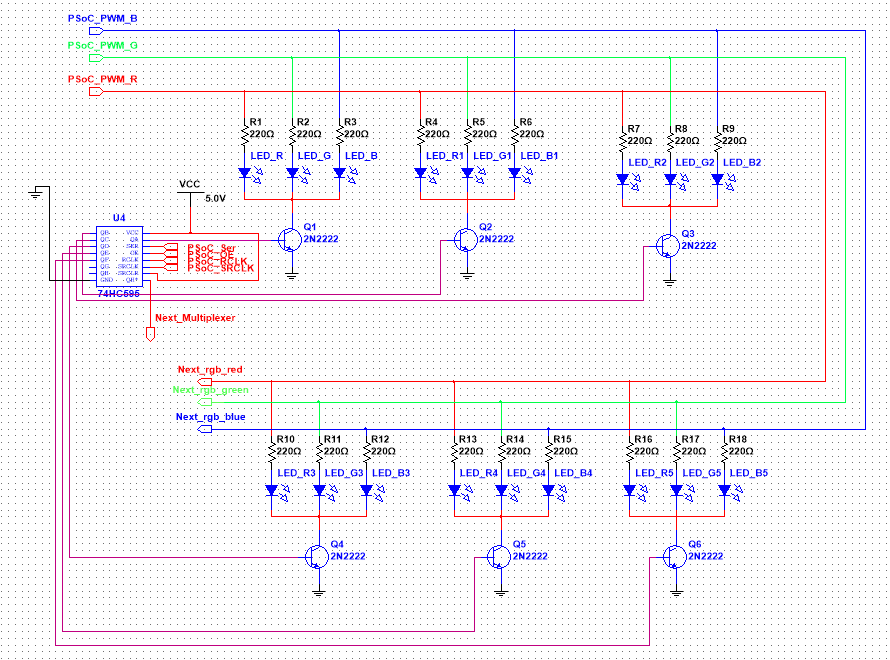
\includegraphics[width=\textwidth]{Softwaredesign/CupLight_IF/graphics/CupLight.png}
    \caption{Design af kontrollen for CupLight}
    \label{fig:CupLight_HW}
\end{figure}

\section{CupLight\_IF Software Design}
Til at kontrollere lyset, der skal være under kopperne, skal der bruges en driver. Dette kapitel vil præsentere nogle af de design valg, der er lavet vedrørende lyset under kopperne.

Da pointen ved at bruge en RGB-led er, at der kan styres farven af led'en så laves der derfor et modul \textit{rgb\_led}, som har til formål at stå for at håndtere det farve mæssige i en RGB-led. Som sagt kan farven på en RGB-led styres ved at bruge PWM på benene, så derfor skal den kunne styre 3 pwm generatorer i PSoC creator. Tilhørende til dette modul laves en typedef struktur kaldet \textit{color\_t}, der er en definition af hvad farverne indeholder (rød,grøn og blå). Farverne hertil kan også kun have værdier mellem 0 og 255, hvilkes der bør tages hånd om i farvernes setMetoder.

\\Denne metode kan i sig selv styre bare en LED, og bør derfor passende testes for dette. I princippet kan den også styre flere LED'er, men dette er ikke relevant til beerpong bordet, da alle LED'er vil have samme farve.

\\Til kontrol af flere LED'er bruges PSoC's SPI Master komponent, da denne kan bruges til at shifte ting ind i et shift register. Derudover skal der være et digital output pin, der har til formål at latche outputtet og et pin, der har til formål at enable outputtet på 74hc595. Det samlede design for komponenterne, der er anvendt i PsoC'en kan ses på figur \ref{fig:CupLight_PSoC_Design}.
\begin{figure}[H]
    \centering
    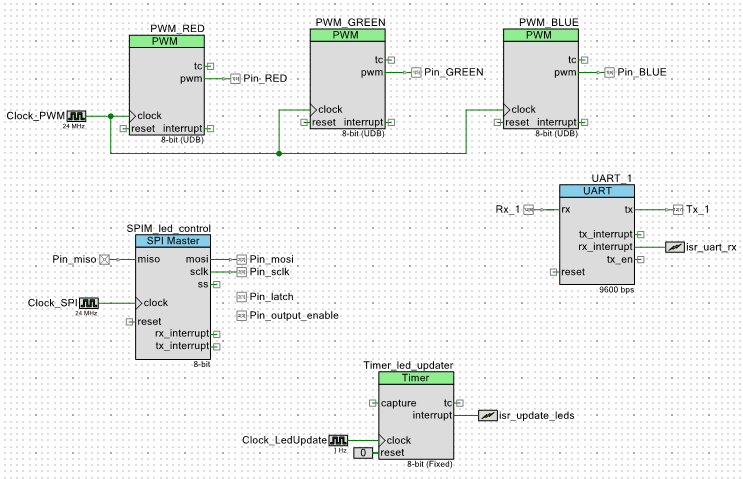
\includegraphics[width=\textwidth]{Softwaredesign/CupLight_IF/graphics/CupLightPSoCDesign.png}
    \caption{PSoC design for CupLight\_IF}
    \label{fig:CupLight_PSoC_Design}
\end{figure}


\end{document}